\section{State of the art}

Quite surprisingly, there is not much work on model-based planning and learning from high-dimensional observations, like images, in complex environments, like video games. This chapter starts with review of state-of-the-art model-free methods that can solve complex tasks like playing video games. Afterwards, the focus moves on to model-based methods that help arrive at the final solution of this thesis problem.

\subsection{World Models} \label{Sec.WorldModels}

In World Models \cite{Algo.WorldModels} paper, a simple model inspired by human cognitive system is used. The authors explore the idea of using large and highly expressive neural networks to reinforcement learning. The RL algorithm is often bottlenecked by the credit assignment problem, which makes it hard for traditional RL algorithms to learn millions of weights of a large model. \\
To avoid this problem, the authors decompose the agent training into two stages: a world model and Controller. The world model, composed of Vision and Memory modules, learns rich spatial and temporal representation of an agent's environment. Thereafter, by using the compressed representation extracted from the world model as inputs to an agent, they train a linear model to perform a task in the environment. The small linear model lets the training algorithm focus on the credit assignment problem on a small search space, while not sacrificing capacity and expressiveness via the larger world model.

In conclusion, their solution consists of three components: Vision for encoding the spatial information, Memory for encoding the temporal information and Controller which represents the agent's policy. Fig.~\ref{Fig.WorldModels} depicts a flow diagram of the agent's model.

\begin{figure}[H]
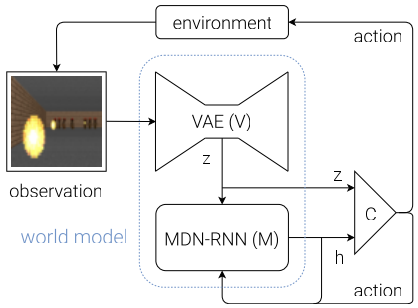
\includegraphics[width=0.7\textwidth,keepaspectratio]{figures/WorldModels.png}
\caption[Flow diagram of the World Models agent's model]{Flow diagram of the agent's model \protect\cite{Algo.WorldModels}. The raw observation is first processed by the Vision (V) at each time step $t$ to produce a latent variable $z_t$. The input into the Controller (C) is the latent variable $z_t$ concatenated with the Memory (M) hidden state $s_t$ at each time step. The Controller will then output an action vector $a_t$ and will affect the environment and produce the next observation. The Memory will then take the current $z_t$ and action $a_t$ as an input to update its own hidden state to produce $s_{t+1}$ to be used at time step $t + 1$.}
\label{Fig.WorldModels}
\end{figure}

This architecture, although quite changed, still reassembles sSSM from the section \ref{Sec.FastWorldModels}. It learns the Memory module in the latent space created by the Vision module. It also explicitly models transitions uncertainty, which will prove to be the key for successful Controller training. What is different though, it predicts the next latent variable conditioned on the next hidden state, $z_{t+1} \sim p(z_{t+1}|s_{t+1})$. The Memory module calculates its next hidden state based on the present hidden state, action and latent variable, $s_{t+1} = f(s_t, a_t, z_t)$. This way, the Memory module is less a sample transition model that predicts one future from all possible futures and more a memory which deterministically encodes facts about the past in the hidden state, which should fully describe the present latent state of the environment, and then use it to sample a latent variable.

The Controller model represents the agent's policy. It is responsible for determining course of actions to take in order to solve a given task. Controller is a simple linear model that maps the concatenated latent variable $z_t$ and hidden state $s_t$ at the time step $t$ directly to the action $a_t$ at that time step.

The authors deliberately made Controller as simple as possible, and trained it separately from Vision and Memory, so that most of the agent's complexity resides in the world model (Vision and Memory). The latter can take the advantage of current advances in deep learning that provide tools to train large models efficiently when well-behaved and differentiable loss function can be defined.
This shift in the agent's complexity towards the world model, as already mentioned, allows the Controller model to stay small and focus its training on tackling the credit assignment problem in challenging RL tasks. It is trained using evolution strategy, which is rather an unconventional choice that only currently have been considered as a viable alternative to popular RL techniques \cite{Algo.ESRL}.

Their solution is able to solve an OpenAI Gym's CarRacing environment \cite{Code.OpenAIGym}, which is the continuous-control racing task, with top-down view on the car and the track. It is the first known solution to achieve the score required to solve this task. Nonetheless, because the Controller uses real experience for training counted in millions of episodes, they did not improve sample-efficiency compared to other model-free solutions \cite{Algo.CarRacingA3C}. But, what is really interesting, in the process of training the Memory learns to simulate the original environment. The authors show that the learned Controller can function inside of the imagined environment of CarRacing, that is, simulated by the Memory.
In the second experiment, they show that the agent can not only play in imagination, but also it is able to learn solely from imagined experience, produced by its Memory, and successfully transfer this policy back to the actual environment of VizDoom (see fig.~\ref{Fig.VizDoom}). In the first trials, the Controller learned to exploit imperfect simulations of the Model, which only approximates the true environment dynamics. To mitigate this behaviour, they adjust the temperature parameter  \cite{Algo.Sketch-RNN} of Memory to control the amount of randomness in the simulation, hence controlling the trade-off between realism and exploitability.
The Controller learns from simulated experience, which means that only tens of thousands of episodes from the environment are needed for the training of Vision and Memory. Assuming that each episode consists of hundreds of frames, millions of frames in total are required for training. It makes World Models very sample efficient compared to other state-of-the-art model-free methods that require even two orders of magnitude more data \cite{Algo.A3C}.

\begin{figure}[H]
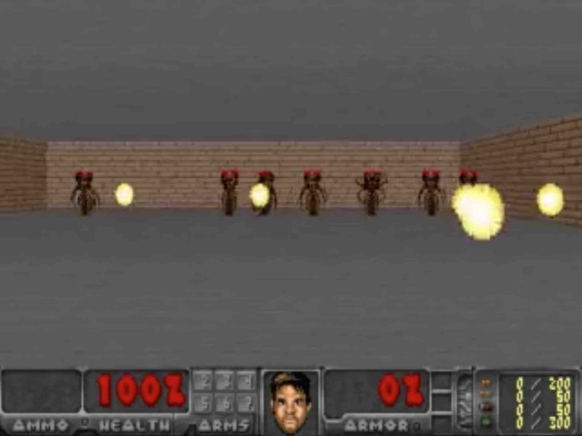
\includegraphics[width=0.7\textwidth,keepaspectratio]{figures/VizDoom.png}
\caption[VizDoom]{VizDoom: the agent must learn to avoid fireballs shot by monsters from the other side of the room with the sole intent of killing the agent \protect\cite{Algo.WorldModels}.}
\label{Fig.VizDoom}
\end{figure}

The authors results indicate that their world model is able to model complex environments from visual observations and it can be used for planning. Therefore, it may prove useful for the topic of this thesis.

\subsection{Learning Latent Dynamics for Planning from Pixels}

In \cite{Algo.PlaNet}, the authors propose the Deep Planning Network (PlaNet), a purely model-based agent that learns the environment dynamics from images and chooses actions through fast online planning in latent space. To achieve high performance, the dynamics model must accurately predict the rewards ahead for multiple time steps. This approach uses a latent dynamics model for its fast querying capabilities, described earlier in the section \ref{Sec.FastWorldModels}. Moreover, they propose a multi-step variational inference objective named latent overshooting already described in the section \ref{Sec.ModelLearning}. The authors found that several dynamics models benefit from latent overshooting, although their final agent, which use the RSSM model described below, does not require it.

Despite its generality, the purely stochastic transitions make it difficult for the transition model to reliably remember information for multiple time steps. In theory, this model could learn to set the variance to zero for some state components, but the optimization procedure may not find this solution. This motivates including a deterministic sequence of activation vectors $\{s_t\}^T_{t=1}$ that allow the model to access not just the last latent variable, $z_{t-1}$, but all previous states deterministically. The authors use such a model, shown in fig.~\ref{Fig.PlaNetModelDesigne}, that they name recurrent state-space model (RSSM). Intuitively, one can understand this model as splitting the state into a stochastic part $z_t$ and a deterministic part $s_t$, which depend on the stochastic and deterministic parts at the previous time step.

\begin{figure}[H]
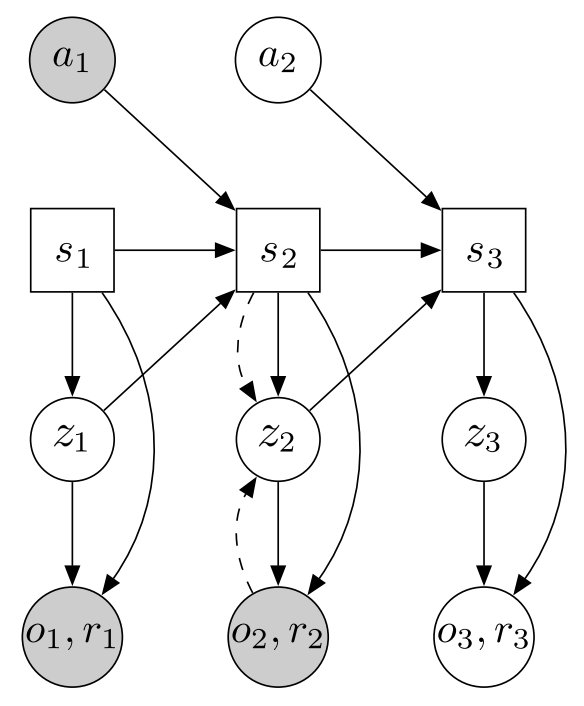
\includegraphics[width=0.5\textwidth,keepaspectratio]{figures/PlaNet/model.png}
\caption[PlaNet latent dynamics model design]{Latent dynamics model design \protect\cite{Algo.PlaNet}. In this example, the model observes the first two time steps and predicts the third. Circles represent stochastic variables and squares deterministic variables. Solid lines denote the generative process and dashed lines the inference model. This model splits the latent state into stochastic and deterministic parts, allowing the model to robustly learn to predict multiple futures.}
\label{Fig.PlaNetModelDesigne}
\end{figure}

Similar to sSSM from the section \ref{Sec.FastWorldModels}, it learns a transition model in latent space for efficiency. This latent dynamics model is designed with both deterministic and stochastic components \cite{Algo.FastGenerativeModels}. Original experiments indicate having both components to be crucial for high planning performance. Like in World Models, it condition a latent variable only on a deterministic state. It calculates the next deterministic state based on the present deterministic state, action and latent variable, $s_{t+1} = f(s_t, a_t, z_t)$ and samples the next latent variable based on the next state, $z_{t+1} \sim p(z_{t+1}|s_{t+1})$. It can be viewed that stochastic part of the state is determined by deterministic part of the state at any time step. This is reversed relationship relative to sSSM and it helps preserve a deterministic part of the state for multiple time steps and this way further improve the simulation accuracy. \\
RSSM also learns an encoder $q(z_t | o_{\leqslant t}, a_{< t})$, observation model $p(o_t | s_t, z_t)$, also called a decoder, and reward model $p(r_t | s_t, z_t)$. The encoder is used to infer an approximate belief over the current latent variable from the history. The observation model provides a rich training signal but is not used for planning.

Given these components, the authors implement the policy as a planning algorithm that searches for the best sequence of future actions. In contrast to model-free and hybrid reinforcement learning algorithms, the authors do not use a policy or value network. \\
The cross entropy method \cite{Algo.CEM} (CEM) is used to search for the best action sequence under the model. The authors decided on this algorithm because of its robustness and because it solved all considered tasks when given the true dynamics for planning. CEM is a population-based optimization algorithm that infers a distribution over action sequences that maximize the sum of rewards for a short future horizon. It uses the model to evaluate sampled candidate sequences in the optimization process. Because the reward is modeled as a function of the latent state, it can operate purely in latent space without generating images, which allows for fast evaluation of large batches of action sequences. After optimization finished, the first action from the resulting sequence is issued to the environment and the process starts from scratch in the next state.

Since the agent may not initially visit all parts of the environment, it iteratively collect new experience and further refine the dynamics model.

Using only pixel observations, PlaNet's agent solves continuous control tasks from DeepMind control suite (see fig.~\ref{Fig.DeepMindControlSuite}) with contact dynamics, partial observability, and sparse rewards, which exceed the difficulty of tasks that were previously solved by planning with learned models. PlaNet uses substantially fewer episodes and reaches final performance close to and sometimes higher than strong model-free algorithms.

\begin{figure}[H]
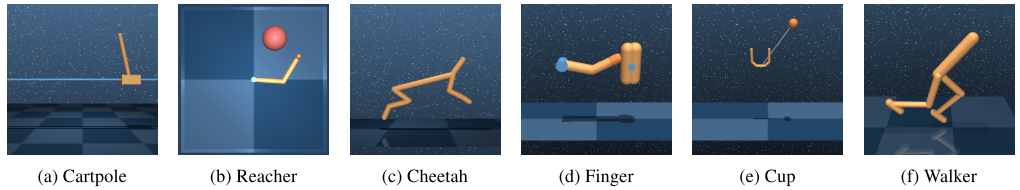
\includegraphics[width=1.0\textwidth,keepaspectratio]{figures/PlaNet/benchmarks.png}
\caption[DeepMind Control Suite]{DeepMind Control Suite: image-based control domains used in PlaNet's experiments \protect\cite{Algo.PlaNet}.}
\label{Fig.DeepMindControlSuite}
\end{figure}

Within 100 episodes, PlaNet outperforms the policy-gradient method A3C \cite{Algo.A3C} trained from proprioceptive states for 100,000 episodes, on all tasks. After 500 episodes, it achieves performance similar to D4PG \cite{Algo.D4PG}, trained from images for 100,000 episodes, except for the finger task. PlaNet surpasses the final performance of D4PG with a relative improvement of 26\% on the cheetah running task.

Moreover, the authors trained a single agent on all six tasks. The agent is not told which task it is facing, it needs to infer this from the image observations. The agent solves all tasks while learning slower compared to individually trained agents. This indicates that the model can learn to predict multiple domains, regardless of the conceptually different visuals.

PlaNet is a working example of a model-based agent that learns a latent dynamics model from high-dimensional image observations and chooses actions by fast planning in latent space. The authors show that their agent succeeds at several continuous control tasks from image observations, reaching performance that is comparable to the best model-free algorithms while using 200 times fewer episodes and similar or less computation time. The results show that learning latent dynamics models for planning in image domains is a promising approach. This thesis will adopt PlaNet to its objectives.

\subsection{Model-Based Reinforcement Learning for Atari}

In \cite{Algo.SimPLe}, the authors explore how video prediction models can enable RL agents to solve Atari games with orders of magnitude fewer interactions than model-free methods. They describe Simulated Policy Learning (SimPLe), a complete model-based deep RL algorithm based on video prediction models, and present a comparison of several model architectures, including a novel architecture that yields the best results in Atari games \cite{Code.ALE}.

SimPLe, apart from an Atari 2600 emulator environment $env$, use a neural network simulated environment $env'$ which they call a world model. The authors find out that crucial decisions in the design of world models are: inclusion of stochasticity, clipping reconstruction loss to a constant and, because simulator $env'$ is supposed to consume its own predictions from previous steps which will be imperfect due to compounding errors, to mitigate a problem of the model drifting out of the area of its applicability they randomly replace in training some frames of the input by the model prediction from the previous step. 

The environment $env'$ shares the action space and reward space with $env$ and produces visual observations in the same format, as it will be trained to mimic $env$. The authors principal aim is to train a policy $\pi$ using a simulated environment $env'$ so that $\pi$ achieves good performance in the original environment $env$. Using short rollouts for a policy training is crucial to mitigate the compounding errors problem described in the section \ref{Sec.ModelLearning}. To ensure exploration of further episode states, SimPLe starts training rollouts from randomly selected states taken from the real data buffer.

In this training process the authors aim to use as few interactions with $env$ as possible. The initial data to train $env'$ comes from random rollouts of $env$. As this is unlikely to capture all aspects of the environment, they use the data-aggregation iterative method.

Experiments evaluate SimPLe on a range of Atari games and show that it achieves competitive results compared to model-free baselines with only 100K interactions between the agent and the environment, which corresponds to about two hours of real-time play. SimPLe is significantly more sample-efficient than a highly tuned version of the state-of-the-art Rainbow algorithm \cite{Algo.Rainbow} on almost all games. In particular, in low data regime of 100k samples, on more than half of the games, SimPLe achieves a score which Rainbow requires at least twice as many samples. In the best case of Freeway, it is more than 10x more sample-efficient.

SimPLe is a similar approach to model-based RL like in World Models. The authors train the dynamics model and use it to generate new experience, the same as in World Models, but in observations space, opposite to World Models. \\
Although this thesis share the goal of sample efficient RL via model-based planning and learning in complex environments, like Atari games, with SimPLe, it tries to accomplish it in fundamentally different way. The thesis solution focuses on training accurate transitions model in the latent state-space to enable fast simulation and search using this model. Pixel-perfect reconstructions are not a concern.

\subsection{Value Prediction Network}

Paper \cite{Algo.VPN} proposes a novel deep reinforcement learning architecture, called Value Prediction Network (VPN), which integrates model-based planning and model-free learning of reward and value functions into a single neural network. In contrast to typical model-based RL methods, VPN learns the dynamics model of an abstract state space sufficient for predicting future rewards and values, rather than future observations. \\
In order to train VPN, the authors propose a combination of temporal-difference search \cite{Algo.TDSearch} and n-step Q-learning \cite{Algo.A3C}. In brief, VPN learns to predict values via Q-learning and rewards via supervised learning. At the same time, VPN perform lookahead planning to choose actions during play and compute target Q-values during training.

VPN has the ability to simulate the future and plan based on the simulated future abstract-states. Although many existing planning methods (e.g. MCTS) can be applied to the VPN, the authors implement a simple planning method which rollout trajectories using the VPN up to a certain depth and aggregates all intermediate value estimates as described in the paper \cite{Algo.VPN}. The planning procedure estimates the current state Q-values which an agent uses to decide on the next action.

Experimental results show that VPN has several advantages over both model-free and model-based baselines in a stochastic navigation task where careful planning is required but building an accurate observation-prediction model is difficult. Furthermore, VPN outperforms Deep Q-Network \cite{Algo.DQN}, strong model-free baseline method, on several Atari games even with short-lookahead planning, demonstrating its potential as a new way of learning a good state representation.

VPN uses an abstract model of rewards to augment model-free learning with good results on a number of Atari games. However, this method does not actually aim to model or predict future environment's states and achieves clear but relatively modest gains in sample-efficiency. On the other hand, it is an example of simple tree search algorithm which can successfully use the learned model for planning, something that this thesis could base on.
